% Template LaTeX file for MInfSem papers
%
% To generate the correct references using BibTeX, run
%     latex, bibtex, latex, latex
% modified...
% - from DAFx-00 to DAFx-02 by Florian Keiler, 2002-07-08
% - from DAFx-02 to DAFx-03 by Gianpaolo Evangelista
% - from DAFx-05 to DAFx-06 by Vincent Verfaille, 2006-02-05
% - from DAFx-06 to DAFx-07 by Vincent Verfaille, 2007-01-05
%                          and Sylvain Marchand, 2007-01-31
% - from DAFx-07 to DAFx-08 by Henri Penttinen, 2007-12-12
%                          and Jyri Pakarinen 2008-01-28
% - from DAFx-08 to DAFx-09 by Giorgio Prandi, Fabio Antonacci 2008-10-03
% - from DAFx-09 to DAFx-10 by Hannes Pomberger 2010-02-01
% - from DAFx-10 to DAFx-12 by Jez Wells 2011
% - from DAFx-12 to DAFx-14 by Sascha Disch 2013
% - from DAFx-14 to MInfSem by Wolfgang Fohl 2014
%
% Template with hyper-references (links) active after conversion to pdf
% (with the distiller) or if compiled with pdflatex.
%
% 20060205: added package 'hypcap' to correct hyperlinks to figures and tables
%                      use of \papertitle and \paperauthorA, etc for same title in PDF and Metadata
%
% 1) Please compile using latex or pdflatex.
% 2) If using pdflatex, you need your figures in a file format other than eps! e.g. png or jpg is working
% 3) Please use "paperftitle" and "pdfauthor" definitions below

%------------------------------------------------------------------------------------------
%  !  !  !  !  !  !  !  !  !  !  !  ! user defined variables  !  !  !  !  !  !  !  !  !  !  !  !  !  !
% Please use these commands to define title and author of the paper:
\def\papertitle{Is it a bird? Is it a plane? It's...\protect\\ \vspace{2 mm} {\small An overview over object recognition problems and advances with regard to the requirements of Open Source Intelligence.}}
\def\paperauthorA{Lotte Steenbrink}


%------------------------------------------------------------------------------------------
\documentclass[twoside,a4paper]{article}
\usepackage{minfsem}
\usepackage{amsmath,amssymb,amsfonts,amsthm}
\usepackage{euscript}
\usepackage[latin1]{inputenc}
\usepackage[T1]{fontenc}
\usepackage{ifpdf}

\usepackage[english]{babel}
\usepackage{caption}
\usepackage{subfig, color}

\usepackage{hyperref}
\usepackage[pdftex]{graphicx}
\usepackage[figure,table]{hypcap}

%=== lottes changes ===
\usepackage{todonotes}
\usepackage{wrapfig}

% Glossary benutzen
\usepackage{glossaries}
\loadglsentries[main]{glossary}
\makeglossaries

\setcounter{page}{1}
\ninept

\usepackage{times}
% Saves a lot of ouptut space in PDF... after conversion with the distiller
% Delete if you cannot get PS fonts working on your system.

% pdf-tex settings: detect automatically if run by latex or pdflatex
\newif\ifpdf
\ifx\pdfoutput\relax
\else
   \ifcase\pdfoutput
      \pdffalse
   \else
      \pdftrue
\fi

%\ifpdf % compiling with pdflatex
%  \usepackage[pdftex,
%    pdftitle={\papertitle},
%    pdfauthor={\paperauthorA},
%    colorlinks=false, % links are activated as colror boxes instead of color text
%    bookmarksnumbered, % use section numbers with bookmarks
%    pdfstartview=XYZ % start with zoom=100% instead of full screen; especially useful if working with a big screen :-)
%  ]{hyperref}
%  \pdfcompresslevel=9
%  \usepackage[pdftex]{graphicx}
%  \usepackage[figure,table]{hypcap}
%\else % compiling with latex
%  \usepackage[dvips]{epsfig,graphicx}
%  \usepackage[dvips,
%    colorlinks=false, % no color links
%    bookmarksnumbered, % use section numbers with bookmarks
%    pdfstartview=XYZ % start with zoom=100% instead of full screen
%  ]{hyperref}
  % hyperrefs are active in the pdf file after conversion
%  \usepackage[figure,table]{hypcap}
%\fi

\title{\papertitle}

%--------------AUTHOR HEADER STARTS -----------------------
\affiliation{
\paperauthorA}
{\href{http://www.haw-hamburg.de/ti-i}{Hamburg University of Applied Sciences,
    Dept. Computer Science,} \\ Berliner Tor 7\\ 20099 Hamburg, Germany\\
{\ttfamily \href{mailto:lotte.steenbrink@haw-hamburg.de}{lotte.steenbrink@haw-hamburg.de}}
}
%-----------------------------------AUTHOR HEADER ENDS------------------------------------------------------

\begin{document}
% more pdf-tex settings:
\ifpdf % used graphic file format for pdflatex
  \DeclareGraphicsExtensions{.png,.jpg,.pdf}
\else  % used graphic file format for latex
  \DeclareGraphicsExtensions{.eps}
\fi

\maketitle

\begin{abstract}
\todo{go into Open Source Intelligence}
Recognizing an categorizing objects in an image is one of the problems which are harder to solve for computers than for humans. However, image recognition is imperative to make human-computer interaction more natural and improve the way information contained in images is stored and handled. In recent years, the field has seen a lot of progress. This paper aims to provide an overview over the challenges faced by image recognition software, and available solutions as well as their limitations.
\end{abstract}


\section{Introduction}
\label{sec:intro}
%===============================================================================



The term \emph{\gls{OSINT}} describes publicly accessible information which has been gathered, processed, exploited, analyzed and grouped in order to support a specific mission.\todo{source, except for handbook of intelligence?}
While this information can be gathered from anywhere, including newspaper, radio or TV reports, public registries \todo{mehr analogweltbeispiele}, the Internet has grown to be a fruitful source of OSINT. Communication has moved online, and, in part, into the public eye, with people debating on twitter, facebook or through their own blogs. Users display their knowledge and interests on their public profiles and help sites such as StackExchange or Quora, post their resumé on LinkedIn and track and document their lives with the help of fitness apps, Instagram, swarm.app, flickr, YouTube, yelp, and many more. Even with more prohibitive privacy settings, researchers can oftentimes extract metadata from the traces a person's online activity leaves:\\
Through nickname reuse, full identities can be reconstructed even from seemingly anonymous interactions. Even if a facebook profile is not public, access to its friend lists and their fried lists reveals information about social structures and cliques which can be identified through \gls{SNA}. Twitter can be searched for \@-mentions to a public profile, reconstructing the contents of a tweet from the public reactions to it.\\ \todo{what about grindr, tinder? what about privacy policies?}
The ability to sift through pictures, tag, classify and put them into context automatically would pose a big step forward for the accumulation of OSINT.
<nette ueberleitung>



\begin{figure}[h!]
\centering
    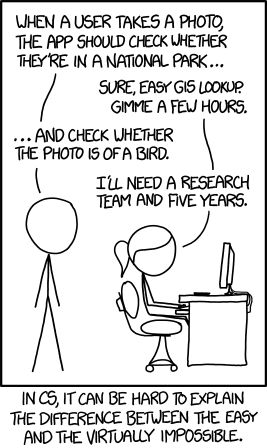
\includegraphics[width=0.3\textwidth]{images/xkcd}
\caption{TODO}
\label{fig:xkcd}
\end{figure}
% three types: 1. die präsenz eines bestimmten(!) objekts/objektart zu erkennen in einem bild (detection), 2. die position eines bestimmten(!) objekts/objektart zu finden (localization)  oder z.b. auch 3. rauszufinden was für eine objektart den grade da ist (categorisation? da sind diese convolutional neural nets super drin. das ist aber superschwierig und deep learning ist da grade state of the art)


% neingeist: ABER: detection wird auch häufig wie meine defintion von localization benutzt (also “where is $objectclass”)

The research field of \emph{Computer Vision} aims to teach computers how to understand images and video footage. This involves recognizing, locating and classifying the objects shown, and understanding the context they're in.
%The task of locating and identifying an object in an image is widely referred to as \emph{Object recognition}.
While this is a relatively easy task for humans, computers still struggle with this as of today. Understanding an image can be divided into different subtasks, some of which rely on each other:
% There are several subfields that make up the umbrella term of ``Object recognition''. some of which rely on each other:
\begin{description}
\item[Object detection] Is there a chair in this image?
\item[Object identification:] Is that a chair?
\item[Object localization:] Where is the chair in this picture?
\item[Object categorization:] Does this image contain furniture?
\item[Image classification:] What is this picture about?
\end{description}

Significant leaps have been made in the subfield of face and human detection and recognition: Consumer-grade cameras have been able to detect smiles and faces for more than a decade now \todo{quelle}, and reliable face recognition is hardly news in both surveillance\todo{src: biometric cams} and civil\todo{src facebook, apple/iphoto face recognition} applications.\todo{what about govt/agency tools?}
The recognition of other objects, however, nevertheless poses a significant challenge. Over the course of this paper, challenges to both object detection and computer vision-aided OSINT gathering will be discussed.

The rest of this paper is organized as follows. TODO

\section{Computer Vision Challenges}
\label{sec:object_det}
%===============================================================================
In some subtasks, computer vision capabilities are starting to compare to human abilities. Other subtasks still remain unreliable even with state-of-the-art approaches, often requiring novice readers to adjust their expectations in terms of what may be considered ``exceptionally good performance''.\footnote{See \url{http://abstrusegoose.com/496} for a humorous depiction of this process.} % idee: die comic panels zur strukturierung?
This section will go into the different tasks mentioned in section \ref{sec:intro}, discussing specific challenges for this type of image processing, and pointing towards state-of-the-art solutions. 

\subsection{Object detection}
\label{sec:object_det}
%...............................................................................


\subsection{Object identification}
\label{sec:object_id}
%...............................................................................
The human brain is able to recognize objects with astonishing precision. As \cite{liter_or_into} points out, humans will have no problem recognizing all but one chair in fig. \ref{TODO: add pic} are of the same make, even though they are captured at different angles. The tiny chair on top of the table will be obvious as decoration and the shadow on the wall will be obvious to be just that-- a shadow, not a piece of furniture.

For a computer, this is fairly less obvious.\todo{elaborate}

Neural Networks, siehe u.a.
http://code.flickr.net/2014/10/20/introducing-flickr-park-or-bird/

\subsubsection{Object vs. Face Recognition}
\label{subsec:object_vs_face}
%...............................................................................

Even with different lighting, a different environment and angle, humans are able to tell with 97,5\% precision whether two pictures show the same person\cite{Taigman_2014_CVPR}\todo{find firsthand source}\todo{same measurements for objects?}.



\subsection{Object categorization}
\label{sec:object_cat}
%...............................................................................


\subsection{Object localization}
\label{sec:object_loc}
%...............................................................................

\subsection{Image classification}
\label{sec:img_cls}
%...............................................................................
Image Classification is defined as the process of looking at an image and classifying it into a set of categories\cite{forsyth2012computer} based on the content of the image. The most common applications for this process are the filtering of sexually explicit images. which may be forbidden by legislation or workplace policies, and preventing the placement of ads near content that the target audience may find distressing.


\section{Computer Vision in practice}
\label{sec:zusammenhang}
%===============================================================================

Flickr park or bird, facebook things, @interesting\_jpg (womit wird das gemacht?)

- govt vs civil applications?

\section{OSINT applications and requirements for Computer Vision}
\label{sec:osint_req_app}
%===============================================================================

OSINT can, in capable hands, be a powerful tool. \todo{Praxisbeispiel recherche}
Who uses OSINT?
\emph{For government agencies}, OSINT can add context to classified information.\\
\emph{law enforcement}
- political groups
- pen testers\cite{unauth_access}; security community in general
- journalists
- doxxing asshats? ()

\subsection{OSINT requirements}
\label{subsec:osint_req}
%...............................................................................
%but!
%- ansprüche höher weil fehler folgenschwerer als zB bei facebook
%- OSINT zum proaktiven ausspaehen (siehe folien) problematisch

When used for OSINT tools, no matter by whom, computer vision results have to satisfy much higher expectations than in civil, everyday use. Being wrongly tagged in a photo on facebook is a nuisance at worst. But, as \cite{derosa2004data} points out, the same mistake made by a government agency tool may seriously impact the falsely targeted person's life, including stigmatization, wrongful prosecution or even the endangering of lives.\\
Even without the monopoly on legitimate use of force, journalists or political activists are able to wreak havoc in a person's life.\\

% problemstellung doxxing, verdachtslose verwendung von OSINT?

\subsection{OSINT applications}
\label{subsec:osint_app}
%...............................................................................

Worauf laeuft das ganze hinaus? bilderdatenbanken, klassifiziert nach KOntext etc? Bestehende Daten schneller durchsuchen? Was für hilfsmittel nehmen wir dafür?

TODO: Fokus liegt a nicht auf face recognition/detection, sondern auf \emph{object recognition/detection}-- wofür könnte das OSINT-technisch nützich sein?


\subsection{Conclusion}
\label{subsec:conclusion}
%...............................................................................
- how can civil computerviz be used to gain intelligence? what's problematic about that? who has access to these tools?
- what can govt agencies do with OSINT + computerviz that civilians can't?


\newpage
\printglossary

\nocite{*}
\bibliographystyle{IEEEbib}
\bibliography{minfsem_tmpl} % requires file minfsem_tmpl.bib


\end{document}
